%%%%%%%%%%%%%%%%%%%%%%%%%%%%%%%%%%%%%%%%%%%%%%
%Includes + Defines
%%%%%%%%%%%%%%%%%%%%%%%%%%%%%%%%%%%%%%%%%%%%%%

%\usepackage{color, colortbl}
%\usepackage{trfsigns}
%\usepackage{graphicx}
%\definecolor{TabularBackgroundColor}{rgb}{0.83,0.96,0.96}
%\usepackage{mathrsfs}


%%%%%%%%%%%%%%%%%%%%%%%%%%%%%%%%%%%%%%%%%%%%%%
%Content
%%%%%%%%%%%%%%%%%%%%%%%%%%%%%%%%%%%%%%%%%%%%%%
\section{Integraltransformationen}

\subsection{Faltung}
\begin{multicols}{2}

  $$y(t) = (x_1 * x_2)(t) = \int \limits _{-\infty} ^{\infty} x_1(\tau) \cdot x_2(t-\tau) d\tau$$
  \textbf{Eigenschaften:} \\
  \begin{tabular}{cc}
    Kommutativ  & ($f * g = g * f$)         \\
    Assoziatiov & ($(f*(g*h)) = ((f*g)*h)$) \\
    Distributiv & ($f*(g+h)= f*g + f*h$)    \\
    Stetigkeit  & ist \textbf{immer} stetig
  \end{tabular}

  \subsubsection*{Vorgehen}
  \begin{enumerate}
    \item $\tau$ bzw. $t-\tau$ in die Entsprechende Funktion Einsetzen
    \item Bereiche Bestimmen an denen die Funktion $\neq 0$
    \item Bereiche bzw. eingesetzte Funktionen in Hilfsdiagramm einzechnen (siehe Bsp.)
    \item Einzelne Integrationsbereiche mit Hilfe Diagramm bestimmen,
          indem Zeit $t$ "raufgezählt" und übergänge der Grenzen beachtet wird
    \item Integrale Bestimmen, Integralgrenzen = Eingezeichnete Grenzen im Diagramm.
    \item Integrale auflösen
  \end{enumerate}
  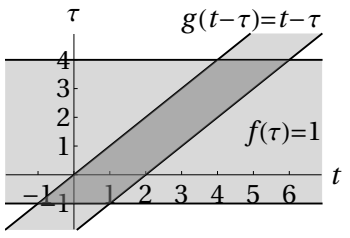
\includegraphics[width = 4.5cm]{include/Integraltransformationen/img/Faltungsgrenzen.png}
  \\\textbf{Beispiel}
  \\$f(t)= \begin{cases}
    2 \textrm{ für } 0 <t<4 \\
    0 \textrm{ sonst}
  \end{cases}
  g(t) = \begin{cases}
    3 \textrm{ für } 0<t<1 \\
    0 \textrm{ sonst}
  \end{cases}$
    \\1.$(f * g)(t) \int \limits _{-\infty} ^{\infty} f(\tau)g(t-\tau)d\tau$
    \\2.  $f(t): 0<\tau<4g(t): 0<t-\tau<1 \Rightarrow t-1 < \tau < t$
    \\3.  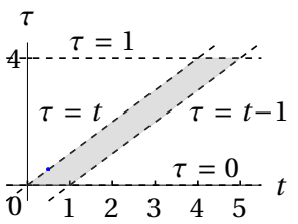
\includegraphics[width = 2cm]{include/Integraltransformationen/img/Bsp_Grenzen.png}
    \\4. und 5. $(f*g)(t) =$
    \\$t \leq 0: 0$
  \\$0 < t \leq 1: \int \limits _0 ^t 2 \cdot 3 d\tau$
    \\$1<t \leq 4: \int \limits _{t-1} ^t 2\cdot 3 d\tau$
  \\$4 <t \leq 5: \int \limits _{t-1} ^4 2\cdot 3 d\tau$
    \\$5< t: 0$

\end{multicols}


\subsection{Fourier-Reihe und Transformation}
\subsubsection*{Fourier-Reihe}
\begin{tabular}{p{4.5cm}p{11.5cm}}
  Trigonometrische Form    &
  $x(t) = \frac{a_0}{2} + \sum \limits _{n = 1} ^{\infty} a_n \cdot cos(2\pi n f_0 \cdot t) + b_n \cdot sin(2\pi n f_0 \cdot t) $
  \newline $a_n = \frac{2}{T} \int \limits _{T} x(t) dt$
  \newline $a_n = \frac{2}{T} \int \limits _{T} x(t) \cdot cos(2\pi n f_0 \cdot t)dt$
  \newline $b_n = \frac{2}{T} \int \limits _{T} x(t) \cdot sin(2\pi n f_0 \cdot t)dt$
  \\
  \rowcolor{TabularBackgroundColor}
  Harmonische Form         &
  $x(t) = r_0 + \sum \limits _{n = 1} ^{\infty} r_n \cdot cos(2\pi n f_0 \cdot t + \varpi_n)$
  \newline $r_0 = \frac{u_0}{2} = \frac{1}{T} \int  \limits _{T} x(t) dt $
  $r_n > 0 = \sqrt{u_n^2 + v_n^2}$
  $\varphi = arg(u_n - j \cdot v_n) $
  \\
  Komplexe Form            &
  $x(t) = \sum \limits _{n= -\infty} ^{\infty} c_n \cdot e^{jn2\pi f_0 \cdot t}$
  \newline $c_n =\overline{c_{-n}} = \frac{1}{T} \int \limits _{0} ^{T} x(t) \cdot e^{-j n 2 \pi f_0 \cdot t} dt$
  \newline $ 2\pi f_0$ wird auch als \textbf{Kreisfrequenz}  $\omega$ bezeichnet, \newline $f_0$ = Frequenz des Grundsignals $x(t)$.
  \\
  \rowcolor{TabularBackgroundColor}
  Umrechnung Koeffizienten &
  $c_n =\overline{c_{-n}} = \frac{a_n - jb_n}{2} (n = 0,1,2,3,..., b_0 =0)$
  \newline $a_n = 2 \cdot Re(c_n); \; b_n = -2 \cdot Im(c_n) (n = 0,1,2,3,..., b_0 =0)$ \\
\end{tabular}

\begin{multicols}{2}

  \subsubsection*{Fouriertransformation $\mathcal{F}(\omega)$}
  $$ X(\omega) = \mathcal{F}[x(t)] = \int \limits _{-\infty} ^{+\infty} x(t) \cdot e^{-j \omega t} dt $$
  $$ x(t) = \mathcal{F}^{-1}[X(\omega)] = \frac{1}{2 \pi} \int \limits _{- \infty} ^{+ \infty} X(\omega) \cdot e^{j \omega t} d\omega$$
  Rechenregeln Siehe Anhang.


  \subsubsection*{Spektraldarstellung}
  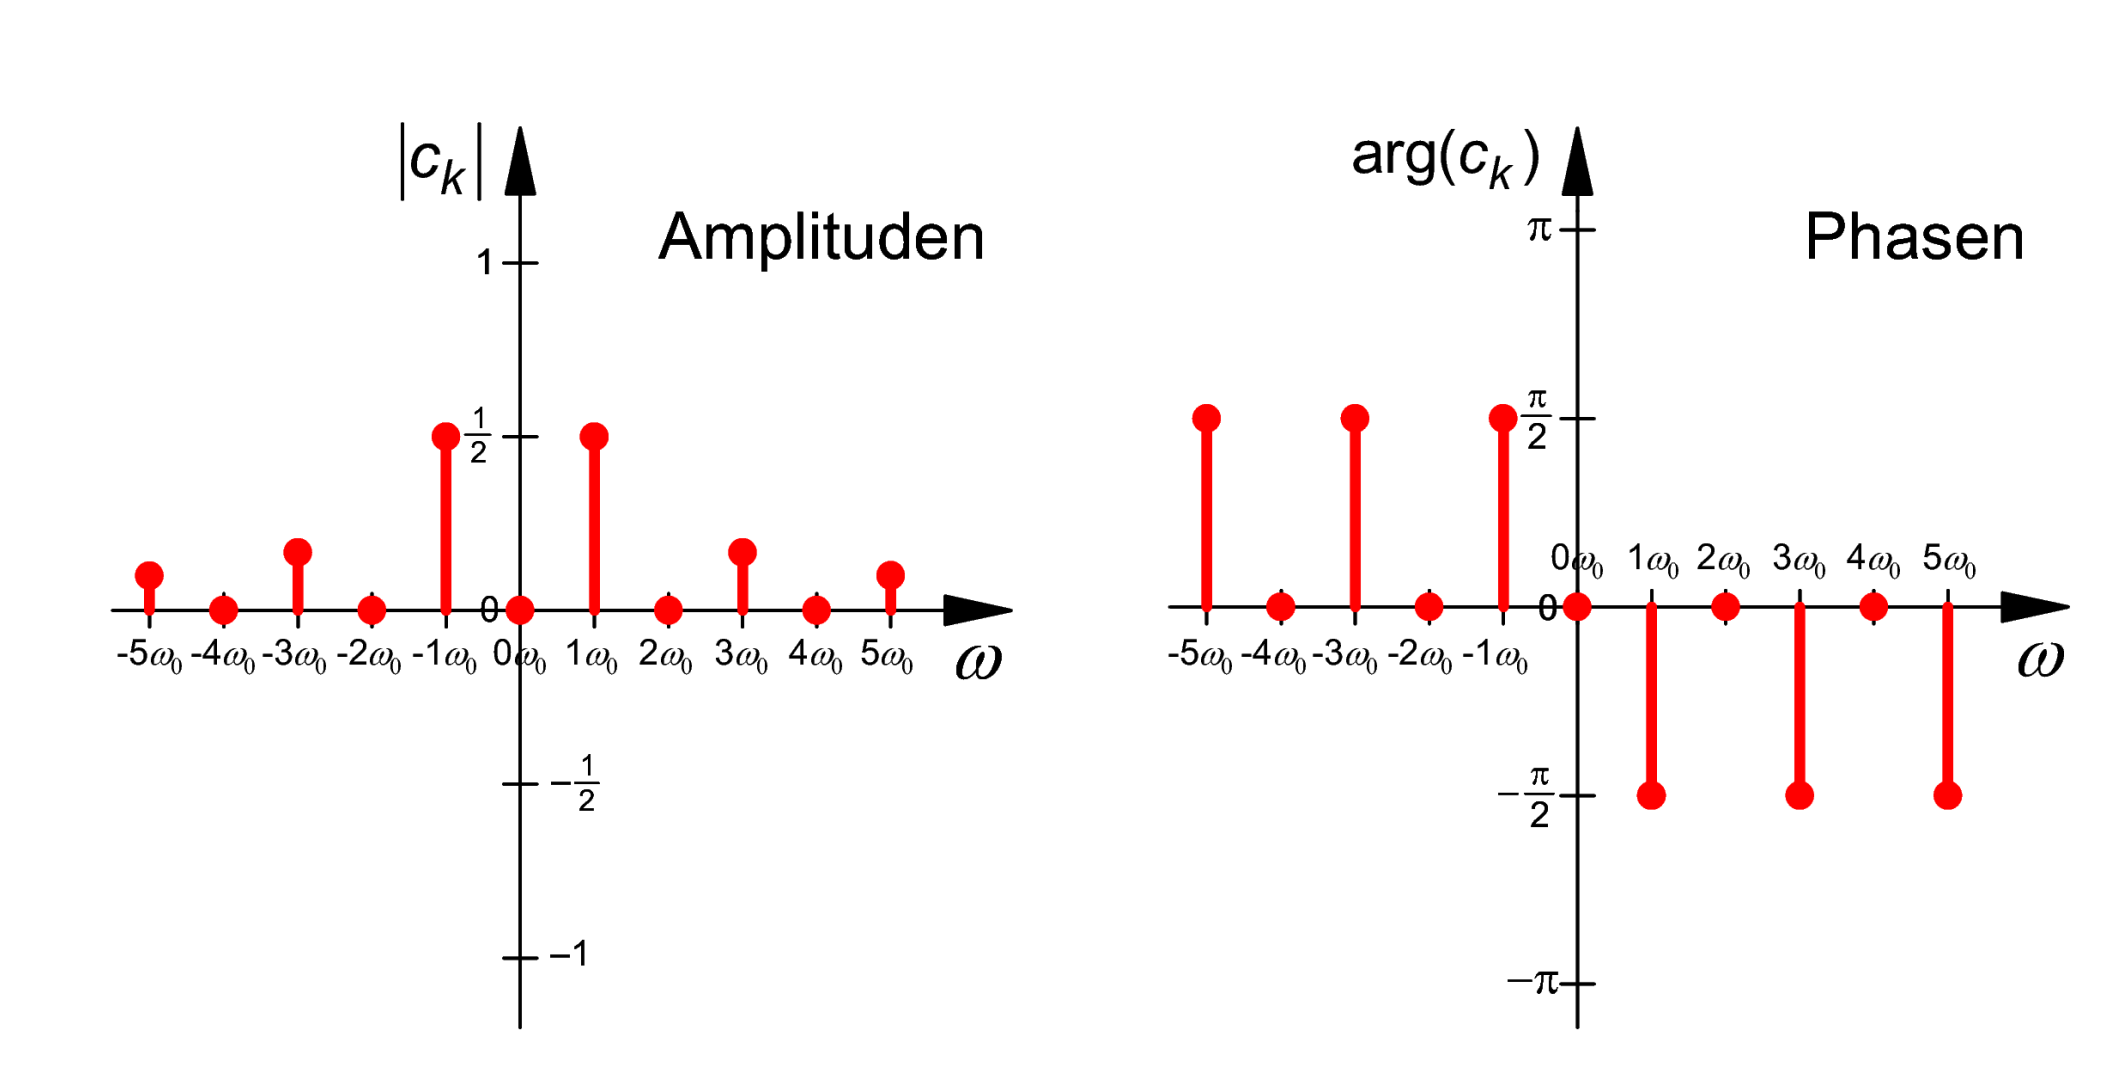
\includegraphics[width = 6cm]{include/Integraltransformationen/img/Spektrum.png}
\end{multicols}

\subsection{Laplace-Transformation}
\begin{multicols}{2}

  $$F(s) = \mathscr{L} {f(t)} = \int \limits _{0} ^{\infty} f(t) \cdot e^{-st} dt \textrm{ mit } s \in \mathbb{C}$$
  $$f(t) = \mathscr{L}^{-1} {f(t)} = \frac{1}{2\pi j} \int \limits _{p_0-j\infty} ^{p_0 + j\infty} F(s) \cdot e^{st} ds$$
  Rechenregeln Siehe Anhang.
  \subsubsection*{Lineare Differenzialgleichungen lösen:}
  DGL in Bildbereich Transformieren \\ $\Rightarrow$ DGL ist jetzt lineare Gleichung
  \\Gleichung auflösen
  \\Lösung Rücktransformieren

  \subsubsection*{Zusammenhänge}
  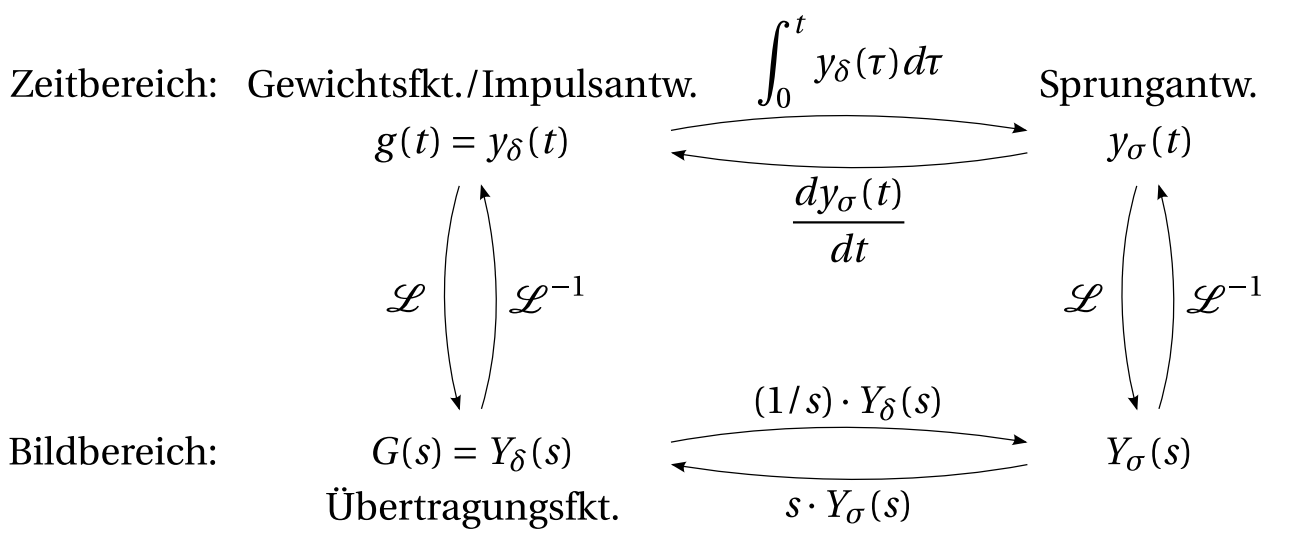
\includegraphics[width = 7cm]{include/Integraltransformationen/img/Zusammenhang_Laplace.png}

  \subsubsection*{Konvergenzhalbebene}
  Die Konvergenzhalbebene beginnt bei der Polstelle der Laplace-Transformierten mit dem Grössete Realteil und geht bis unendlich.
  \newline Bsp: Bei $\frac{1}{s-2}$ ist die Polstelle bei $+2$, daraus folgt: Konvergenzhalbebene $= [2,\infty)$
\end{multicols}

\subsection{Hilbert-Transformation}
\begin{multicols}{2}
  Im \textbf{Zeitbereich:}
  $$\hat{x}(t) = x(t) * \frac{1}{\pi t} = \frac{1}{\pi} \int \limits _{-\infty} ^{\infty} \frac{x(\tau)}{t-\tau} d\tau$$
  Im \textbf{Frequenzbereich}:
  $$\hat{X}(\omega) = X(\omega) \cdot H(\omega) = -j \cdot sgn(\omega) \cdot X(\omega)$$
\end{multicols}
